\documentclass{article}
\usepackage[utf8]{inputenc}
\usepackage{times}
\usepackage[titletoc]{appendix}
\usepackage{graphicx}
\usepackage{lineno}
\usepackage{multirow}
\usepackage[english]{babel}
\usepackage{typearea} 
\usepackage{amssymb}
\usepackage{amsfonts}
\usepackage{amsmath}
\usepackage{enumerate}
\usepackage{mathtools}
\usepackage{graphicx}
\usepackage{wrapfig}
\usepackage{subcaption}
\usepackage{lscape}
\usepackage{rotating}
\usepackage[numbers]{natbib}
\usepackage[colorinlistoftodos]{todonotes}
\usepackage{float}
\usepackage{times}
\newcommand{\Fig}[1]{Figure~\ref{fig:#1}}

\renewcommand{\baselinestretch}{1.5}
\newcommand{\bbar}[1]{\overline{#1}}

\newcommand\scalemath[2]{\scalebox{#1}{\mbox{\ensuremath{\displaystyle #2}}}}


\usepackage[font={small},labelfont={bf},justification=justified,margin=0.5cm]{caption}

\renewcommand{\thesection}{}
\renewcommand{\thesubsection}{\arabic{section}.\arabic{subsection}}

\usepackage{color}
         \definecolor{darkred}{rgb}{0.9,0,0}
%         \definecolor{darkgreen}{rgb}{0,0.5,0}
         \definecolor{darkblue}{rgb}{0,0,0.75}
%         \definecolor{magenta}{rgb}{0,0,0.75}
\newcommand{\hhone}{(H,H,1)}
\newcommand{\hhtwo}{(H,H,2)}
\newcommand{\hsone}{(H,S,1)}
\newcommand{\hstwo}{(H,S,2)}
\newcommand{\shone}{(S,H,1)}
\newcommand{\shtwo}{(S,H,2)}
\newcommand{\ssone}{(S,S,1)}
\newcommand{\sstwo}{(S,S,2)}

\newcommand{\hhstar}{(H,H,$\star$)}


\usepackage{hyperref}
\definecolor{darkgreen}{rgb}{0.1,0.6,0.3}
\definecolor{darkred}{rgb}{0.6,0.3,0.1}
\hypersetup{
    colorlinks=true,       % false: boxed links; true: colored links
    linkcolor=blue,          % color of internal links (change box color with linkbordercolor)
    citecolor=darkgreen,        % color of links to bibliography
    filecolor=magenta,      % color of file links
    urlcolor= black           % color of external links
}


% remove this before we submit...
\definecolor{greenie}{rgb}{0.1,0.62,0.0}
\definecolor{orange}{rgb}{0.9,0.3,0.0}
\definecolor{deepblue}{rgb}{0.0,0.0,0.7}
\newcommand{\cha}[1]{\textcolor{darkgreen}{(#1)}}


\title{\vspace*{-22mm}\bf Evolutionary Game Theory for Understanding Biological Evolution}
%\author{Chaitanya S. Gokhale$^{1}$, Joseph Bulbulia$^{2,3}$, Marcus Frean$^{4}$\\
%\normalsize $^1$Research Group for Theoretical Models of Eco-evolutionary Dynamics\\
%\normalsize Department of Evolutionary Theory, \\
%\normalsize Max-Planck Institute for Evolutionary Biology, 24306 Pl\"{o}n, Germany, \\
%\normalsize $^2$School of Humanities, Faculty of Arts, University of Auckland, New Zealand \\
%\normalsize $^3$Max Planck Institute for the Science of Human History, Jena, Germany \\
%\normalsize $^4$School of Engineering and Computer Science, \\
%\normalsize Victoria University of Wellington, New Zealand
%}


\date{}

\begin{document}


\linenumbers
\maketitle




\noindent
Keywords: 


\tableofcontents
\section{Introduction}
One of the most important part of evolutionary biology revolves around the basic concept of cooperation. Cooperation is required to build new dimensions of biological organization. Cooperation forms the basis of the emergence of genomes, cells, multi-cellular organisms, social insects and human society. Cooperation implies that selfish replicators are willing to sacrifice a part of their reproductive capacity so that they can assist others \citep{Nowak2006}.
Studies suggest that bacterial colonies which form biofilm require high level of cooperation because secreted extracellular polymeric material is a shared resource and can be advantageous to entire bacterial colonies \citep{Xavier2007}. In case of \textit{Dictyostelium discoideum}, also known as social amoeba, where some of the cells become self-sacrificing to create supportive stalks in which a colony of spores propagates \citep{Medina2024}. Also, social insects showing extreme cooperative specialization whereby workers sacrifice their own reproduction in order to contribute to the overall colony's fitness \citep{Fischman2011}.\\
Despite of having evolutionary advantage, cooperation is quite unfavourable in real world systems because when people have an individual self interest, they would likely exceed the amount of collective resource available (Tragedy of commons) or short-term gain through defection is more tempting in real world scenarios \citep{Rankin2007}.
In the biological context, this effect can lead to the public goods dilemma, which means cooperative interactions produce benefits that are distributed among all group members, defectors can enjoy such benefits without necessarily paying the costs that are involved in their creation. 
Let's take examples of bacterial communities, in an experimental study  \textit{Vibrio cholerae} cheater cells can impose experimental benefits of costly extracellular enzymes synthesized by cooperators by evolutionary time \citep{Schluter2015}, and also in a study it is shown that defector individuals of \textit{Pseudomonas aeruginosa} can avoid the expense of generating the QS signal or the cooperative behaviour that is coordinated by QS and but can use QS signal to propagate \citep{Diggle2007}.\\
Natural selection has five main ways of overcoming this obstacle and favoring cooperation, which are kin selection (cooperation among genetic kins), direct reciprocity (repeated encounters with the same individuals), indirect reciprocity (reputation-based cooperation), network reciprocity (spatial structure constraining interactions), and group selection (disproportionate success of groups).
In this thesis, we're analysing population structure, which can significantly influences the evolutionary dynamics by determining which individual interacts with whom. Real populations aren't well-mixed, instead spatial or social structures create non-random patterns of interaction, that can crucially effect the evolution of cooperation over defection. Structuring population spatially should resolve the cooperation dilemma by using spatial clustering and network reciprocity\citep{Nowak2010}. 
In a paper, Powers, Penn, and Watson demonstrate that the cooperation and population structure co-evolve together in a synergistic way\citep{Powers2011}.
This thesis focuses on population structure as a promising pathway to understand cooperation-defection and to catalyse cooperation, since evolving population structure is a necessary parameter for the stability and evolution of cooperative behaviour. The simplest way to simulate a game in structured population through graphs is simulating the game in square lattice spatial structure.\\
Evolutionary Game Theory is one of the most prominent mathematical framework, which can possibly explain these complex evolutionary dynamics by converting biological behaviours as strategic interacting games, where interaction payoffs determine fitness. Unlike classical game theory, evolutionary game theory focuses on evolution of strategy based on the reproductive success or fitness value. An example of a game in EGT, prisoner's dilemma, demonstrates that collective payoff in case of mutual cooperation is relatively greater than that of mutual defection, but individual defection provides more high payoffs when one plays with a cooperator, dispersing defections in the population.
Evolutionary Game Theory can be applied to different biological systems, starting from fermentation, cellular metabolic cooperation, biofilm formation, antibiotic resistance formation, cancer progression modeled as interaction between healthy and malignant cells or quorum sensing as cooperative interactions preventing exploitation while maintaining beneficial collective actions \citep{Hummert2014}.\\
In this thesis, the evolutionary game theory is used to study how population structure facilitates cooperation in biological systems, and mathematical models and computational simulations are used to study the dynamics of cooperation-defection in the context of various spatial and social organization. This study seeks to contribute to the existing body of knowledge of cooperation in microbial ecology, cellular biology and other different biological systems by combining theoretical predictions with empirical examples to determine why cooperation is evolutionarily stable, and how to catalyse cooperation and to determine its key role in the evolution of biological organization.
Our thesis starts with the discussion of the replicator dynamics or deterministic  dynamics, then proceeds through the stochastic dynamics and the section of evolutionary dynamics in the structured population.

\section{Methodology}
\subsection{Replicator Dynamics}
\label{subsec:Replicator Dynamics}
\subsubsection{Two-player games with two strategies}
\label{subsubsec:Two-player games with two strategies}

Replicator dynamics is one of the possible frameworks that can explain evolutionary dynamics. Replicator dynamics determines how the frequency of different strategies in a population changes over time. We can write the equation used to assess replicator dynamics mathematically. Let's take the frequency of $A$ and $B$ strategies are $x_A$ and $x_B$ and the fitness of each strategy is $f_A$ and $f_B$ and the average fitness of the population is $\bar{f}$. It is a two-player two-strategy game, so we can say $ x_A+x_B=1 $, so we can write that $x_B=1-x_A$ and $x_A=1-x_B$. Let's try to write a payoff matrix,\\
\[
\begin{pmatrix}
& A & B \\
  A & a_1 & a_0 \\
  B & b_1 & b_0
\end{pmatrix}
\]
Now, based on the payoffs, we can write the average fitness of each strategy.
\begin{align}
f_A &=x_A\cdot a_1 + (1-x_A)\cdot a_0 \nonumber\\
f_B &=x_B\cdot b_1 + (1-x_B)\cdot b_0 \nonumber
\end{align} 
Now, to keep the average fitness of the population constant, we can write an equation.
\begin{align}
\bar{f}= (x_Af_A+x_Bf_B)\label{eq:1}
\end{align}
Now, we can substitute this $x_B$ value into the equation \eqref{eq:1}. After substitution, we will get the following equation.
\begin{align}
\bar{f}={x_Af_A+ (1-x_A)f_B}\label{eq:2}
\end{align}
We can write two differential equations for replicator dynamics using the above information.
\begin{align}
\frac{dx_A}{dt} = x_A(f_A - \bar{f}) \nonumber \\
\frac{dx_B}{dt} = x_B(f_B - \bar{f}) \label{eq:3}
\end{align}
Now let's substitute the equation \eqref{eq:2} into the equation \eqref{eq:3}.
\begin{align}
\frac{dx}{dt} &=x_A[f_A-(x_Af_A+(1-x_A)f_B)] \nonumber\\
          &=x_A[f_A-x_Af_A-f_B+x_af_B] \nonumber\\
          &=x_A[(1-x_A)f_A-(1-x_A)f_B] \nonumber\\
          &=x_A(1-x_A)(f_A-f_B) \label{eq:4}
\end{align}
This is for a two-strategy game. If we have $n$ strategies,where $i=1,2,3.....(n-1)$.We can write the following equation.
\[\frac{dx_i}{dt}=x_i[f_i(x)-\bar{f}]\]
What does this equation tell us? 
We can understand that the rate of change with time of the frequency of a certain type depends on the fitness, average fitness of the population, and frequency. From this understanding, we can say that if $f_i(x)-\bar{f}>0$, then the frequency of this type will increase over time, and if $f_i(x)-\bar{f}<0$, the frequency of the type will decrease over time.
Now, we can write the replicator dynamics \eqref{eq:4}.
\[\frac{dx}{dt}=x_A(1-x_A)(f_A-f_B)\]
If we make the change of strategy $A$ constant over time, which means $\frac{dx}{dt}=0$ then we can write the replicator dynamics equation as:
\[x_A(1-x_A)(f_A-f_B)=0\]
Now, if we try to find certain conditions under which $\frac{dx}{dt}$ will be $0$.
We will have three certain conditions, $x=0$, $x=1$, and $f_A=f_B$.
In graphical representation, for the condition $f_A=f_B$, it will make a straight line between $0$ and $1$. If the condition is $f_A>f_B$ then the curve will be over the straight line and if $f_A<f_B$ then the curve will be under the straight line\citep{Bishop1976}.\\
We can calculate the particular frequency where the strategy $A$ becomes abundant from rare or rare from abundant. We can calculate this using the $f_A=f_B$ equation.\\
Let's take this frequency as $x^*$.
As we know, $f_A=f_B$
So we can write,
\begin{align}
&xa_1+(1-x)a_0 =xb_1+(1-x)b_0 \nonumber\\
&x(a_1-a_0)+a_0=x(b_1-b_0)+b_0 \nonumber\\
&x(a_1-a_0-b_1+b_0)=b_0-a_0 \nonumber\\
&x=\frac{b_0-a_0}{a_1-a_0-b_1+b_0} \nonumber
\end{align}
We can write the $x$ as $x^*$
\begin{align}
x^*=\frac{b_0-a_0}{a_1-a_0-b_1+b_0} \label{eq:5}
\end{align}
We get different conditions from this equation.\\
(1) Dominance: It happens when one of the two strategies will be dominant over another, meaning, for example, if $f_A>f_B$, that strategy $A$ will be dominant over strategy $B$. It will be possible if the $a_1>b_1$ and $a_0>b_0$, where $a_1,a_0,b_1,b_0$ are the payoffs of a payoff matrix of a two-player two-strategy game.\\
(2) Co-existence: It happens when one of the two strategies is rare and has an advantage over that. For example, if strategy $A$ is rare, then $f_A>f_B$. If $a$ becomes abundant, it will lose its advantage, so the inequality will be  $f_A<f_B$, and while becoming abundant strategy from rare strategy, there will be an internal equilibrium point, and the equation will be $f_A=f_B$. In this scenario, the player should play the rare strategy. It will be possible if the $a_1<b_1$ and $a_0>b_0$, where $a_1,a_0,b_1,b_0$ are the payoffs of a payoff matrix of a two-player two-strategy game.\\
(3) Bi-stability: A condition where all $A$ and $B$ will be stable. It means that a strategy will get an advantage if it is abundant. For example, if strategy $A$ is abundant, then the inequality will be $f_A>f_B$, and if it becomes rare, then the inequality will be $f_A<f_B$, and there will be an internal equilibria when $f_A=f_B$. For this condition, the player should play the strategy that its opponent is playing. It will be possible if the $a_1>b_1$ and $a_0<b_0$, where $a_1,a_0,b_1,b_0$ are the payoffs of a payoff matrix of a two-player two-strategy game.\\
(4) Neutrality: Now, we have one condition in which both strategies will have the same impact. It does not depend on the change in the strategy. The equation for this strategy is $f_A=f_B$. It will be possible if $a_1=b_1$ and $a_0=b_0$ where $a_1,a_0,b_1,b_0$ are the payoffs of a payoff matrix of a two-player two-strategy  game.\citep{Gokhale2011}.\\
Now, based on the above explained process of replicator dynamics for two players with two strategies, we will explore some games and find their internal equilibrium point.\\
\textbf{Prisoner's dilemma}
\newline
The prisoner's dilemma is a fundamental game in game theory, which represents that two rational individuals might not cooperate, even if it benefits them mutually.\\
The game goes on as two prisoners ($A$ player and $B$ player) are arrested by a policeman and offered some separate deals.\\
There will be mainly three conditions:
\begin{enumerate}
\item If both prisoners cooperate, they will get an equal and moderate amount of sentence.
\item If one prisoner defects, the defector will get no sentence, but the cooperator gets a longer sentence.
\item If both players defect, both will get a lower and equal sentence.
\end{enumerate}
Let's try to write the payoff matrix.
\[
\begin{array}{c|cc}
   & \text{Cooperate (C)} & \text{Defect (D)} \\
  \hline
  \text{Cooperate (C)} & R = 3 & S = 0 \\
  \text{Defect (D)} & T = 5 & P = 1 \\
\end{array}
\]
The general and standard condition for the prisoner' dilemma is $a_1<b_1$ and $a_0<b_0$. As mentioned in the replicator dynamics section, there are three conditions where the value of $dx/dt$ will be $0$. The three conditions are $x=0$, which means only defectors, and $x=1$, which means only cooperators. The internal equilibrium will fulfil the condition of $f_C=f_D$. Let's find the equilibrium point by using the equation \eqref{eq:5} and putting the payoff values into the equation.
\begin{align}
x^*&=\frac{1-0}{3-0-5 +1} \nonumber\\
x^*&= -1 \nonumber
\end{align}
Since $x\in{0,1}$ so there can not exist any internal equilibrium valued $-1$. This states that the entire system will transition to full defection $(x=0)$ over time.
We can plot the graph using Python for the Prisoner's dilemma dynamics.
\begin{figure}[H]
    \centering
    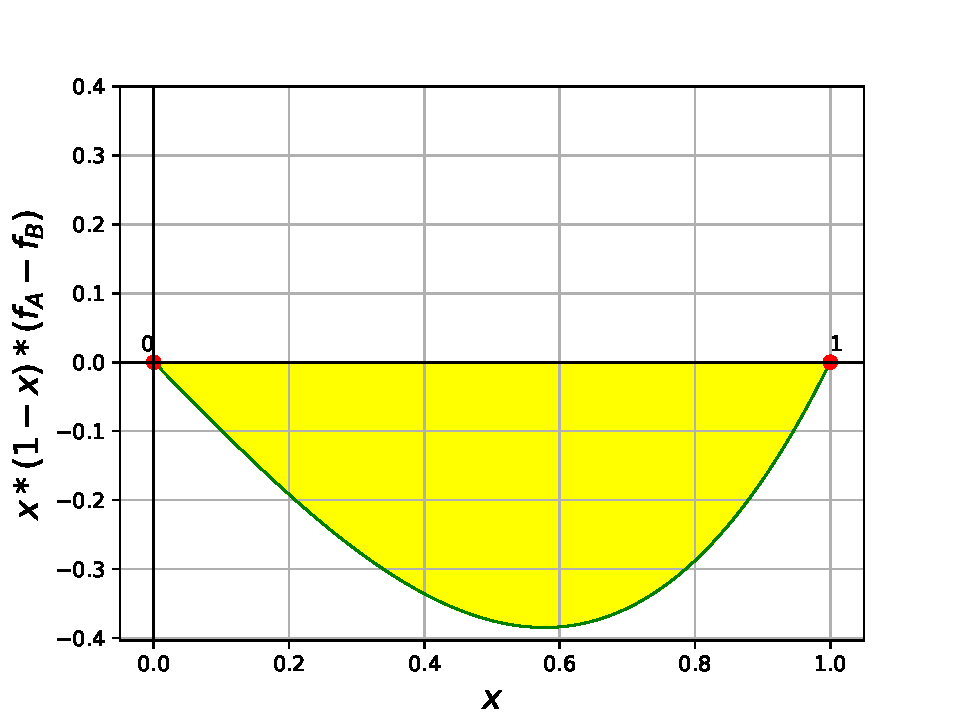
\includegraphics[width=0.6\textwidth]{PD.pdf}
    \caption{$x^*=-1$, Internal Equilibrium for Prisoner's Dilemma Game}
    \label{fig:1}
\end{figure}
\textbf{Chicken Game}
\newline
In this game, two players( player $A$ and player $B$)are driving towards each other on a single pathway. There are two options for the players:
\begin{enumerate}
\item Swerve(C)- Avoided collision but appeared weak.
\item Stay (D)- Stay driving toward each other, hoping the opponent will swerve.
\end{enumerate}
We can write three conditions based on this:
\begin{enumerate}
\item If both swerve, they will not face a collision, but there will be a small loss.
\item If one swerves and one stays, the one who stays will have a win, and the one who swerves will face a loss.
\item If both stay, they'll have a huge loss.
\end{enumerate}
We can write the payoff matrix with actual payoffs, which follow the standard condition, $a_1<b_1$ and $a_0>b_0$.
\[
\begin{array}{c|cc}
   & \text{Swerve} & \text{Stay} \\
  \hline
  \text{Swerve} & -c = -3 & b = 4 \\
  \text{Stay} & 0 = 0 & \frac{b}{2} = 2 \\
\end{array}
\]
As we know, there are three conditions where the value of $\frac{dx}{dt}$ will be $0$. The three conditions are $x=0$, which means only defectors, and $x=1$, which means only cooperators. The internal equilibrium will fulfil the condition of $f_C=f_D$.Let's find the equilibrium point by using the equation \eqref{eq:5} and putting the payoff values into the equation.
\begin{align}
x^*&= \frac{2-4}{-3-4-0+2} \nonumber\\
x^*&= \frac{2}{5} \nonumber
\end{align}
This implies that, over time, $2/5$ of the population will swerve and $3/5$ of the population will stay. It implies the condition of co-existence. Let's try to plot it.
\begin{figure}[H]
    \centering
    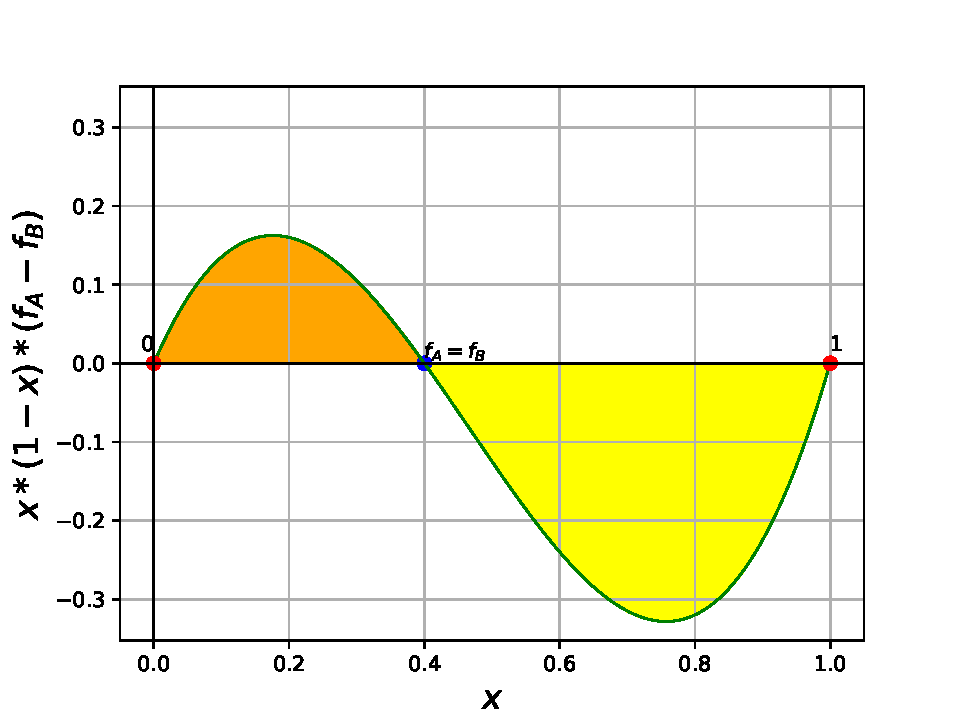
\includegraphics[width=0.6\textwidth]{CG.pdf}
    \caption{$x^*=\frac{2}{5}$, Internal Equilibrium for Chicken Game}
    \label{fig:2}
\end{figure}
\textbf{Stag Hunt Game}
\newline
The stag hunt game is a classical example of game theory for understanding social dilemma and the interplay between risk and trust.
In this game, two players are hunting in a forest. They have two choices: Cooperate(C) with each other and hunt a stag or Independently hunt hare(D).\\
We can write three conditions based on this:
\begin{enumerate}
\item If they both cooperate and hunt stag, they will get the highest payoff.
\item If One goes for the stag hunt and the other one hunts hare, the one who hunts stag will get nothing and the one who hunts hare will get a lower payoff.
\item If they both defect and independently hunt hare, they will get a lower payoff.
\end{enumerate}
We can write the payoff matrix using actual values, which follow the conditions of $a_1>b_1$ and $a_0<b_0$.
\[
\begin{array}{c|cc}
   & \text{Cooperate (C)} & \text{Defect (D)} \\
  \hline
  \text{Cooperate (C)} & S = 5 & S = 1 \\
  \text{Defect (D)} & H = 2 & H = 2 \\
\end{array} \label{eq:6}
\]
As we know, there are three conditions where the value of $dx/dt$ will be $0$. These three conditions are $x=0$, it means only defectors, and $x=1$, which means only cooperators. The internal equilibrium will fulfil the condition of $f_C=f_D$.Let's find the equilibrium point by using the equation \eqref{eq:5} and putting the payoff values into the equation.\\
\begin{align}
x^* &=\frac{2-1}{5-1-2+2} \nonumber\\
x^* &= \frac{1}{4} \nonumber
\end{align}
Over time, $1/4$ of the population will hunt hare and the $3/4$ of the population will hunt stag.
\begin{figure}[H]
    \centering
    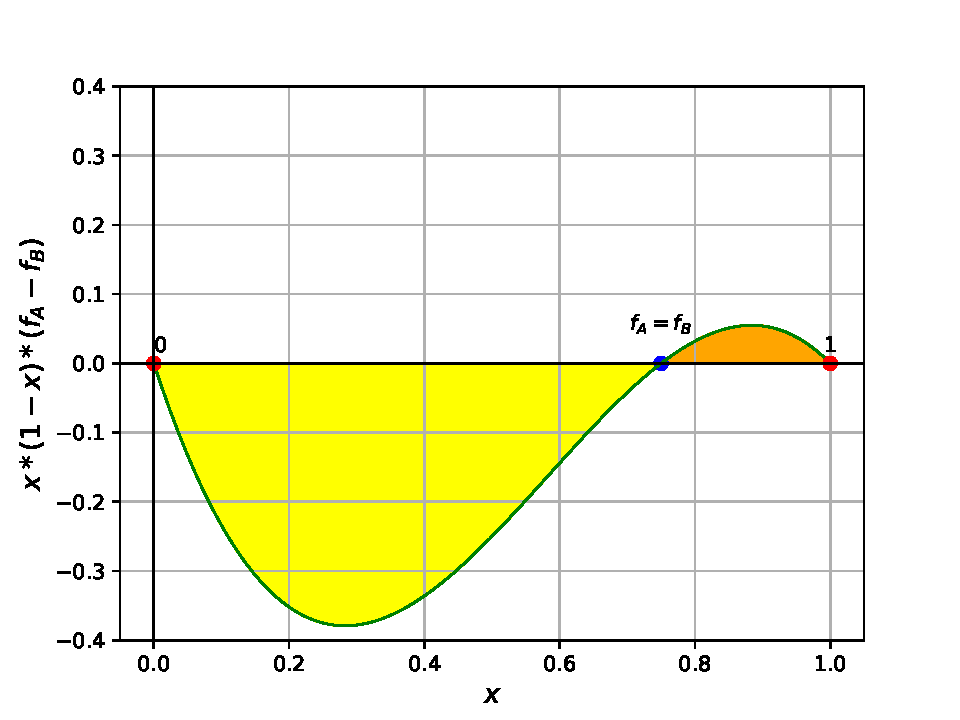
\includegraphics[width=0.6\textwidth]{SH.pdf}
    \caption{$x^*=\frac{1}{4}$, Internal Equilibrium for Stag Hunt Game}
    \label{fig:3}
\end{figure}
\subsubsection{Two player games with multiple strategies}
\label{subsubsec:Two player games with multiple strategies}
In the previous subsection, we analysed two player games with two strategies, now we are going to analyse two player games with multiple strategies. For better understanding of this particular problem, let's take a biological example, strains of \textit{Escherichia coli} are competing for resources available on the media. $K$ strain is the killer strain which produces toxin that will out-compete strain $S$. So, having toxin or not are the two strategies, we can write this using two strategy payoff matrix but there can be another possibility, where strain $R$ is resistant to the toxin but pay the cost for resistance. So, the scenario now changed completely; now the payoff matrix will be $3 \times 3$. This study was carried out by\citep{Kerr2002}\citep{Czaran2002}.
Now, in a population there will be multiple strategies. So, we have to write the replicator dynamics in $(n-1)$ dimensional simplex.For that we need $n\times n$ payoff matrix.
\[
\begin{array}{c@{}c}
   & \begin{array}{cccc} 1 & 2 & \dots & n \end{array} \\ 
   \begin{array}{c} 
       1 \\ 
       2 \\ 
       \vdots \\ 
       n 
   \end{array} 
   & 
   \begin{pmatrix}
       a_{1,1} & a_{1,2} & \dots & a_{1,n} \\
       a_{2,1} & a_{2,2} & \dots & a_{2,n} \\
       \vdots & \vdots & \ddots & \vdots \\
       a_{n,1} & a_{n,2} & \dots & a_{n,n}
   \end{pmatrix}
\end{array}
\] \label{eq:7}
This is a two player game, here $a_{1,2}$ means player $A$ playing strategy $1$ against the strategy $2$ of player $B$ so we can write the equation using replicator dyanmics.
\begin{equation}
dx_i/dt=x_i[f_i(x)-\bar{f}\nonumber\\
\end{equation}
We can derive the average fitness of a strategy $i$ from this equation.
\begin{equation}
f_i(x)=a_{i,1}x_1+a_{i,2}x_2+.....+a_{i,n}x_n\nonumber\\
\end{equation}
We can write this equation as:
\begin{equation}
f_i(x)=\sum_{j=1}^{n}a_{i,j}x_j\nonumber\\
\end{equation}
and the average fitness of a population is denoted as:
\begin{equation}
\bar{f}=x_1f_1+x_2f_2+.....+x_nf_n= \sum_{i=1}^{n}x_if_i\nonumber\\
\end{equation}
\textbf{Rock-Paper-Scissors Game}
\newline
Rock paper scissors game is a game in game theory where, there are $n=3$ strategies for each player. In this game, there are mainly three conditions:
\begin{enumerate}
\item If rock, paper and scissors meet respectively with rock, paper and scissors, the payoff will be zero.
\item If rock meets with scissors and paper with rock and scissors with paper, they will get the highest payoff.
\item If the rock meets with paper and paper with scissors and scissors with rock, they will get the lowest payoff.
\end{enumerate}
Let's try to write the payoff matrix.
\begin{equation}
A =
\begin{pmatrix}
  & R & S & P \\
R & 0 & 1 & -1 \\
S & -1 & 0 & 1 \\
P & 1 & -1 & 0
\end{pmatrix}
\end{equation}
Let's write the average fitness for each strategy,\\
For Rock,
\begin{align}
f_R &= (0)x_R + (1)x_S + (-1)x_P \nonumber\\
f_R &= x_S - x_P \nonumber
\end{align}
For Scissors,
\begin{align}
f_S &= (-1)x_R + (0)x_S + (1)x_P \nonumber\\
f_S &= x_P - x_R \nonumber
\end{align}
For Paper,
\begin{align}
f_P &= (1)x_R + (-1)x_S + (0)x_P \nonumber\\
f_P &= x_R - x_S \nonumber
\end{align}
$x_R,x_S,x_P$ are the frequencies of choosing rock, scissors and paper respectively, and we can write,
\begin{align}
x_R+x_S+x_P=1 \label{eq:8}
\end{align}
Now the mathematical condition for finding the internal equilibrium is $f_R=f_S=f_P$.
\begin{align}
f_R &=f_S \nonumber\\
x_S-x_P &=x_P-x_R \nonumber\\
2x_P &=x_S+x_R \label{eq:9}
\end{align}
\begin{align}
f_S &=f_P \nonumber\\
x_P-x_R &=x_R-x_S \nonumber\\
2x_R &=x_P+x_S \label{eq:10}
\end{align}
\begin{align}
f_R&=f_P \nonumber\\
x_S-x_P&=x_R-x_S \nonumber\\
2x_S&=x_R+x_P \label{eq:11}
\end{align}
Now if we replace the value of \eqref{eq:7} into the equation \eqref{eq:6} we will get,
\begin{align}
x_R+x_S+x_P&=1\nonumber\\
2x_P+x_P&=1\nonumber\\
x_P&=\frac{1}{3}\nonumber
\end{align}
If we replace the value of \eqref{eq:8} and \eqref{eq:9} into the equation \eqref{eq:6} in the same manner, we will get $x_P=x_R=x_S=\frac{1}{3}$. In this game no player will gain an advantage by changing their strategies.
\begin{figure}[H]
    \centering
    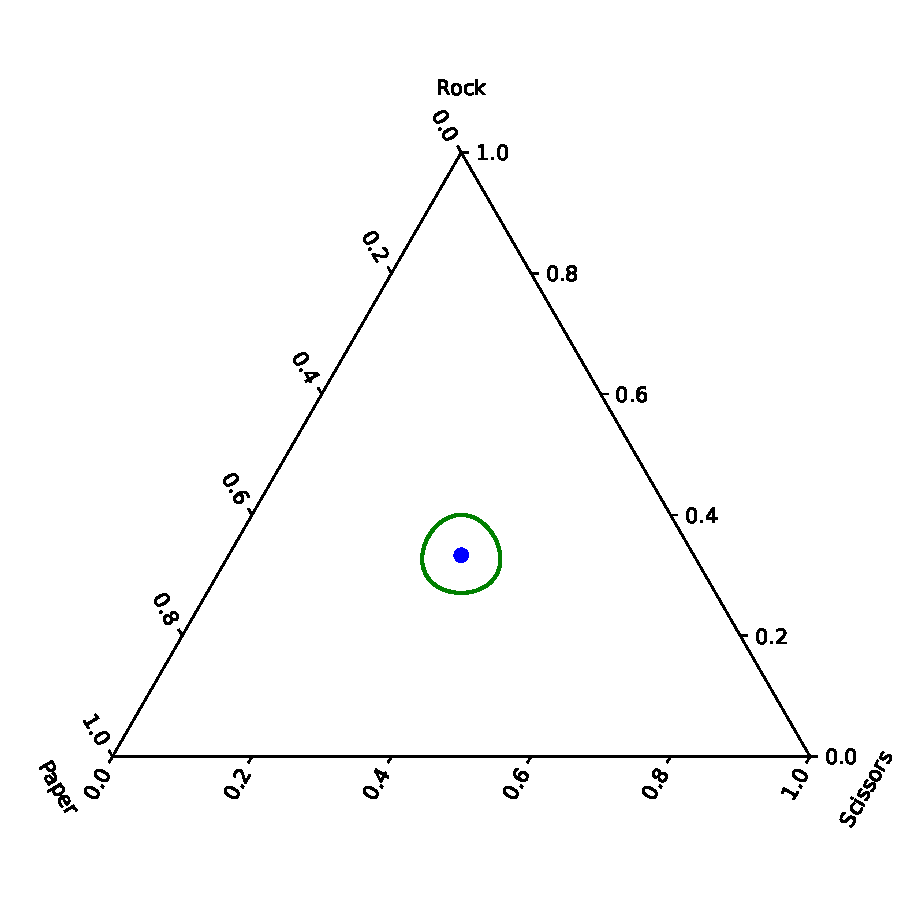
\includegraphics[width=0.6\textwidth]{RPS.pdf}
    \caption{Internal Equilibrium of Rock-Paper-Scissors Game}
    \label{fig:4}
\end{figure} 
\subsection{Stochastic Dynamics and Finite Population}
\subsubsection{Two players with two strategies}
In the previous subsection, we used an infinite population for the deterministic approach \citep{Hofbauer2003}.
Now, we will proceed with a finite population.
There are mainly two reasons to use a finite population: first, it is realistic, and second, it is a natural way to introduce randomness into the replicator dynamics \citep{Altrock2010}.\\
\textbf{Wright-Fisher Process}
\newline
The theory of Wright-Fisher process is rooted in the population genetics. In Wright-Fisher process,each of $N$ individuals in a generation reproduce a large number of offspring which is proportional to their fitness.
From this offspring pool, a $N$ sized generation is again randomly sampled. The composition of the population can change more faster. In principle, in a single generation, the population can go back to a single ancestor. 
It states that the Wright-Fisher process is not a simple birth-death process. It is a more general Markov chain process \citep{Imhof2006}.\\
\textbf{Moran Process}
\newline
Moran process is a classical model of population genetics like Wright-Fisher process. In contrast to the Wright-Fisher process, Moran process is a simple birth-death process, where in a population one randomly selected individual reproduce it's identical copy proportional to it's fitness value and to keep the population size constant one randomly selected individual is removed from the population.
In the previous works, we used trivial fitness means the average fitness is exactly equal to the average payoff. But in the actual population, fitness can depend on payoff in many other ways. For some systems we may know the exact relation between payoff and fitness but for other systems, we can just speculate.
Nowak et al.\citep{Nowak2004} introduced a tunable parameter as selection intensity. 
\begin{equation}
f_i=1-w+w\pi_i \label{eq:12}
\end{equation}
where $f_i$ is the average fitness of a population, $w$ is the selection intensity, $\pi_i$ is the average payoff of a strategy. If $w=1$ it will be strong selection, $f_i=\pi_i$ and if $w=0$ it will be weak selection, $f_i=1$.\\
Now, we can consider the finite population of a specific game as $N$.
Let's assume there are two strategies $A$ and $B$. Number of players playing strategy $A$ and $B$ are $j$ and $(N-j)$ respectively.
We can write the payoff matrix according to this specification.
\[
\begin{array}{c|cc}
    & A & B \\
    \hline
  A & a_1 & a_0 \\
  B & b_1 & b_0
\end{array}
\]
Now we can denote the average payoff of $a$ and $b$ strategies as $\pi_a$ and $\pi_b$.
\begin{align}
\pi_A&=\frac{j-1}{N-1}a_1 + \frac{N-j}{N-1}a_0 \nonumber\\
\pi_B&=\frac {j}{N-1}b_1 + \frac{N-j-1}{N-1}b_0\label{eq:13}
\end{align}
Now, a question can arise, why are we using $N-1$ instead of $N$? We have to understand that instead of an infinitely large population, we are using a real finite population and for that, we have to remove the particular individual who is observing or analysing the situation, so we use $N-1$.\\
Now, we can move to the part of the evolutionary dynamics for the finite population where randomness is involved in the population.
So, we will go for the stochastic processes.
For these stochastic processes, we will focus on the Moran process. It consists of two events: birth and death. 
For the birth process, one subject is chosen randomly, and it produces its identical copy, and for the death process, again, one random subject is chosen from the population and eliminated. 
It means by introducing randomness with the birth-death process, now this theory can change the population with each time step, and for $N$ steps it will control a generation \cite{Moran1962}
There are three situations in this theory.
\begin{enumerate}
\item The number of individual playing strategy $A$ increases by 1.
\item The number of individual playing strategy $A$ decreases by 1.
\item The number of individual playing strategy $A$ remains neutral.
\end{enumerate}
From these three scenarios we can write there equations.\\
For the (1) scenario,
\begin{equation}
T_j^+=\frac{jf_A}{jf_A+(N-j)f_B}\frac{N-j}{N} \label{eq:14}
\end{equation}
For the (2) scenario,
\begin{equation}
T_j^-=\frac{(N-j)f_A}{jf_A+(N-j)f_B}\frac{j}{N} \label{eq:15}
\end{equation}
For the (3) scenario,
\begin{equation}
1-T_j^+-T_j^- \label{eq:16}
\end{equation}
Now, what can we tell from these equations?
\begin{enumerate}
\item From the \eqref{eq:12} equation, we can say that  individual playing strategy $A$ can increase only when an individual playing strategy $A$  is chosen for birth and an individual playing strategy $B$  is chosen for death.
\item From the \eqref{eq:13} equation, we can say that the number of the individuals playing strategy $A$ decreases because an individual playing strategy $A$ individual is chosen for death and an individual playing strategy $B$ is chosen for birth.
\item From the \eqref{eq:14} equation, we can deduce that no one is chosen for the birth or death process, so there is neutrality.
\end{enumerate}
\textbf{Fixation Probability}
\newline
In genetics, we often ask a question related to the invasion of a gene: how can the gene invade another gene, and how does it affect the other gene's population?
After understanding the transition probability and Moran processes, we can now form a question based on the previously mentioned topic.
In a population of $j$ numbered individuals playing strategy $A$ and $(N-j)$ numbered individuals playing strategy $B$, what is the probability of the whole population will consist of individuals playing $A$?
This is known as the fixation probability of $j$ numbered individuals playing $A$ strategy.
We can denote this fixation probability as $\rho_j$.
The two absorbing states are $\rho_j=0$ and $\rho_j=1$.
Since fixation is an absorbing state, if the entire population once becomes $A$, it can not be reverted. We can try to write a probability balance equation.
\begin{align}
\rho_j &= T_j^-\rho_{j-1}+(1-T_j^+ - T_j^-)\rho_j + T_j^+p_{j+1} \nonumber\\
0 &= T_j^-\rho_{j-1} - T_j^-\rho_j - T_j^+\rho_j + T_J^+\rho_{j+1}\nonumber\\
0 &= \underbrace{-T^-_j (\rho_j - \rho_{j-1})}_{y_j} + \underbrace{T^+_j (\rho_{j+1} - \rho_j)}_{y_{j+1}} \label{eq:17}
\end{align}
We can write this equation as the differences between fixation probabilities, $y_{j+1}=y_jr_j$, where $r_j=\frac{T_j^-}{T_j^+}$
\begin{align}
y_1 &= \rho_1 - \rho_0 = \rho_1 \nonumber\\
y_2 &= \rho_2 - \rho_1 = r_1 \rho_1 \nonumber\\
\vdots \nonumber\\
y_k &= \rho_k - \rho_{k-1} = \rho_1 \prod_{j=1}^{k-1} r_j \label{eq:18}\\
\vdots \nonumber\\
y_N &= \rho_N - \rho_{N-1} = \rho_1 \prod_{j=1}^{N-1} r_j \label{eq:19}
\end{align}
This means each incremental change from $\rho_{N-1}$ to $\rho_N$ is based on the growing product of $r_j$ multiplied by $\rho_1$.\\
Now let's calculate the sum over all $y_j$. This sum is telescopic sum.
\begin{align}
\sum_{k=1}^N y_k &= \rho_1-\rho_0+ \rho_2-\rho_1+ \rho_3-\rho_2+\cdots+\rho_N-\rho_{N-1} \nonumber\\
\sum_{k=1}^N y_k &= \rho_N-\rho_0=1 \label{eq:20}
\end{align}
Using \eqref{eq:16} and \eqref{eq:18} we can calculate the value of $\rho_1$.
\begin{equation}
1=\sum_{k=1}^N y_k=\sum_{k=1}^N \rho_1 \prod_{j=1}^{N-1}r_j=\rho_1(1+ \sum_{k=1}^{N-1}\prod_{j=1}^k r_j)\label{eq:21}
\end{equation}
So, we can write the fixation probability of one $A$ individual as,
\begin{equation}
\rho_1= \frac{1}{1+ \sum_{k=1}^{N-1}\prod_{j=1}^k r_j} \label{eq:22}
\end{equation}
For neutral selection, $T_j^-=T_j^+$ and $r_j=1$. Hence, all products are simply one and we find $\rho_1= 1/N$.\\
This is the fixation probability of single mutant $\rho_1$. In general, the fixation probability of $i$ mutants are $\rho_i$.
\begin{align}
\rho_i&= \sum_{k=1}^i y_k \nonumber\\
&= \rho_1 \sum_{k=1}^i \prod_{j=1}^{k-1}r_j\nonumber\\
&=\rho_1(1+ \sum_{k=1}^{i-1} \prod_{j=1}^k r_j)\nonumber\\
&= \frac{1+\sum_{k=1}^{i-1}\prod_{j=1}^k r_j}{1+ \sum_{k=1}^{N-1}\prod_{j=1}^k r_j} \label{eq:23}
\end{align}
For neutral selection, we have $T_j^-=T_j^+$ and $r_j=1$. Hence, all products are simply one and we find $\rho_1= j/N$.\\
The probability that a single individual playing strategy $A$ takes over a population of $N-1$ individuals playing strategy $B$ is the fixation probability of strategy $A$, $\rho_A=\rho_1$.\\
The probability that a single individual playing strategy $B$ takes over a population of $N-1$ individuals playing strategy $A$ is the fixation probability of strategy $B$. The fixation probability of $B$ strategy is equal to the $N-1$ individuals playing strategy $A$ fail to take over the population so there is only one individual playing strategy $B$. So, the fixation probability of strategy $B$ is $\rho_B= 1-\rho_{N-1}$.\citep{traulsen2009stochastic}
\begin{align}
\rho_B &=1-\rho_{N-1} \nonumber\\
&=\frac{1 + \sum_{k=1}^{N-2} \prod_{j=1}^{k} r_j}{1 + \sum_{k=1}^{N-1} \prod_{j=1}^{k} r_j} \nonumber\\
&= \frac{1 + \sum_{k=1}^{N-1} \prod_{j=1}^{k} r_j}{1 + \sum_{k=1}^{N-1} \prod_{j=1}^{k} r_j} - \frac{1 + \sum_{k=1}^{N-2} \prod_{j=1}^{k} r_j}{1 + \sum_{k=1}^{N-1} \prod_{j=1}^{k} r_j} \nonumber\\
&= \frac{\prod_{j=1}^{N-1} r_j}{1 + \sum_{k=1}^{N-1} \prod_{j=1}^{k} r_j} \nonumber \\
&= \rho_A \prod_{j=1}^{N-1} r_j \label{eq:24}
\end{align}
\textbf{Weak Selection and Risk Dominance}
\newline
For weak selection, selection intensity is $w\ll 1$ and $r_j$ simplifies to,
\begin{equation}
r_j = \frac{1-w+w\pi_B}{1-w+w\pi_A} \approx 1-w(\pi_A-\pi_B) \label{eq:25}
\end{equation}
Now we can write the product in the \eqref{eq:21} in a simplified way for weak selection.
\begin{equation}
\prod_{j=1}^k r_j \approx \prod_{j=1}^k 1-w(\pi_A-\pi_B) \approx 1-w \sum_{j=1}^k (\pi_A-\pi_B). \label{eq:26}
\end{equation}
Now, let's annotate a equation $(\pi_A-\pi_B)$.
From equation \eqref{eq:13} we can write,
\begin{align}
\pi_A - \pi_B &= \frac{(j - 1)a + (N - j)b - jc - (N - j - 1)d}{N - 1} \nonumber\\
&= \frac{j(a - b - c + d) + (-a + bN - dN + d)}{N - 1}\nonumber\\
&= \underbrace{\frac{a - b - c + d}{N - 1}}_{u} j 
+ \underbrace{\frac{-a + bN - dN + d}{N - 1}}_{v} \label{eq:27}
\end{align}
Now, let's solve the sum for the payoff difference using equation \eqref{eq:27}.
\begin{equation}
\sum_{j=1}^{k} (\pi_A - \pi_B) = \sum_{j=1}^{k} (u j + v) = u \frac{(k+1)k}{2} + vk = \frac{u}{2}k^2 +( \frac{u}{2} + v)k. \label{eq:28}
\end{equation}
Now, the ratio of fixation probabilities:
\begin{align}
\frac{\rho_B}{\rho_A} &= \prod_{j=1}^{N-1}r_j \approx 1 - w \sum_{j=1}^{N-1} (\pi_A - \pi_B)\nonumber\\
&= 1 - w[ \frac{u}{2}(N-1) + \frac{u}{2} + v](N-1) \nonumber\\
&= 1 - \frac{w}{2} \underbrace{[(a - b - c + d)(N - 1) - a - b - c + 3d + (2b - 2d)N]}_{\Xi} \label{eq:29}
\end{align}
If the payoff difference is $\Xi > 0$, then only strategy $A$ will be favoured, means $\rho_A>\rho_B$.
For large population, $N \gg 1$ we can write that
\begin{equation}
0<\Xi \approx N(a+b-c-d)\label{eq:30}
\end{equation}
It is equivalent to
\begin{equation}
x^*=\frac{d-b}{a-b-c+d}<\frac{1}{2} \label{eq:31}
\end{equation}
So, we can write that $\rho_A >\rho_B$ is equivalent to $x^*<\frac{1}{2}$.
This condition is risk dominance and it implies that for weak selection, strategies which have higher fixation probabilities can invade and fixate from a wider range of starting conditions.\\
\textbf{One-Third Rule}
\newline
Now we can write the approximation of the fixation probability equation under weak selection by inserting equation \eqref{eq:28} into equation \eqref{eq:22}.
\begin{align}
\rho_1 &= \frac{1}{1+\sum_{k=1}^{N-1} \prod_{j=1}^{k}r_j}\nonumber\\
&\approx \frac{1}{1+\sum_{k=1}^{N-1}[1-w(\frac{u}{2}k^2+(\frac{u}{2}+v)k)]} \label{eq:32}
\end{align}
If we use the formula $\sum_{k=1}^{N-1} k = \frac{N(N - 1)}{2}$ and $\sum_{k=1}^{N-1} k^2 = \frac{N(N - 1)(2N - 1)}{6}$, the fixation probability will be,
\begin{align}
\rho_1 &\approx\frac{1}{(N - 1)- w [\frac{u}{2}\frac{N(N - 1)(2N - 1)}{6} + (\frac{u}{2} + v)\frac{N(N - 1)}{2}]}\nonumber\\
&\approx \frac{1}{N - w[ u \frac{N(N - 1)(2N - 1)}{12} + ( \frac{u}{2} + v)\frac{N(N - 1)}{2}]}\nonumber\\
&\approx \frac{1}{N - wu \cdot \frac{N(N - 1)(2N - 1)}{12} - w ( \frac{u}{2} + v)\frac{N(N - 1)}{2}} \nonumber\\
&= \frac{1}{N} + \frac{w}{4N}[\underbrace{( a - b - c + d)\frac{2N - 1}{3} - a - b - c + 3d + (2b - 2d)N
}_{\Gamma}] \label{eq:33}
\end{align}
Now take this condition for $w=0$ which is known as neutral selection.
Neutral selection means there is no selective force working, and the fixation is totally determined by randomness.
So, in the case of neutral selection the fixation probability $\rho_1 = \frac{1}{N}$.
Now, if we want to know that if the fixation probability is higher than $\frac{1}{N}$ or not, we need to consider $\Gamma$.
If $\Gamma>0$ then only fixation probability will be greater than $\frac{1}{N}$.
\begin{equation}
\frac{a-b-c+d}{3}+ b-d > 0 \label{eq:34}
\end{equation}
The condition showed in the \eqref{eq:34} is equivalent to,
\begin{equation}
x^* = \frac{d-b}{a-b-c+d}<\frac{1}{3} \label{eq:35}
\end{equation}
This condition is known as one-third rule.
It implies that the fixation probability of a strategy will be higher than $\frac{1}{N}$, meaning the strategy is more likely to fix than by random drift, if and only if the unstable tipping point $x^*$ is less than $\frac{1}{3}$ \citep{Ohtsuki2007}.
\begin{figure}[H]
    \centering
    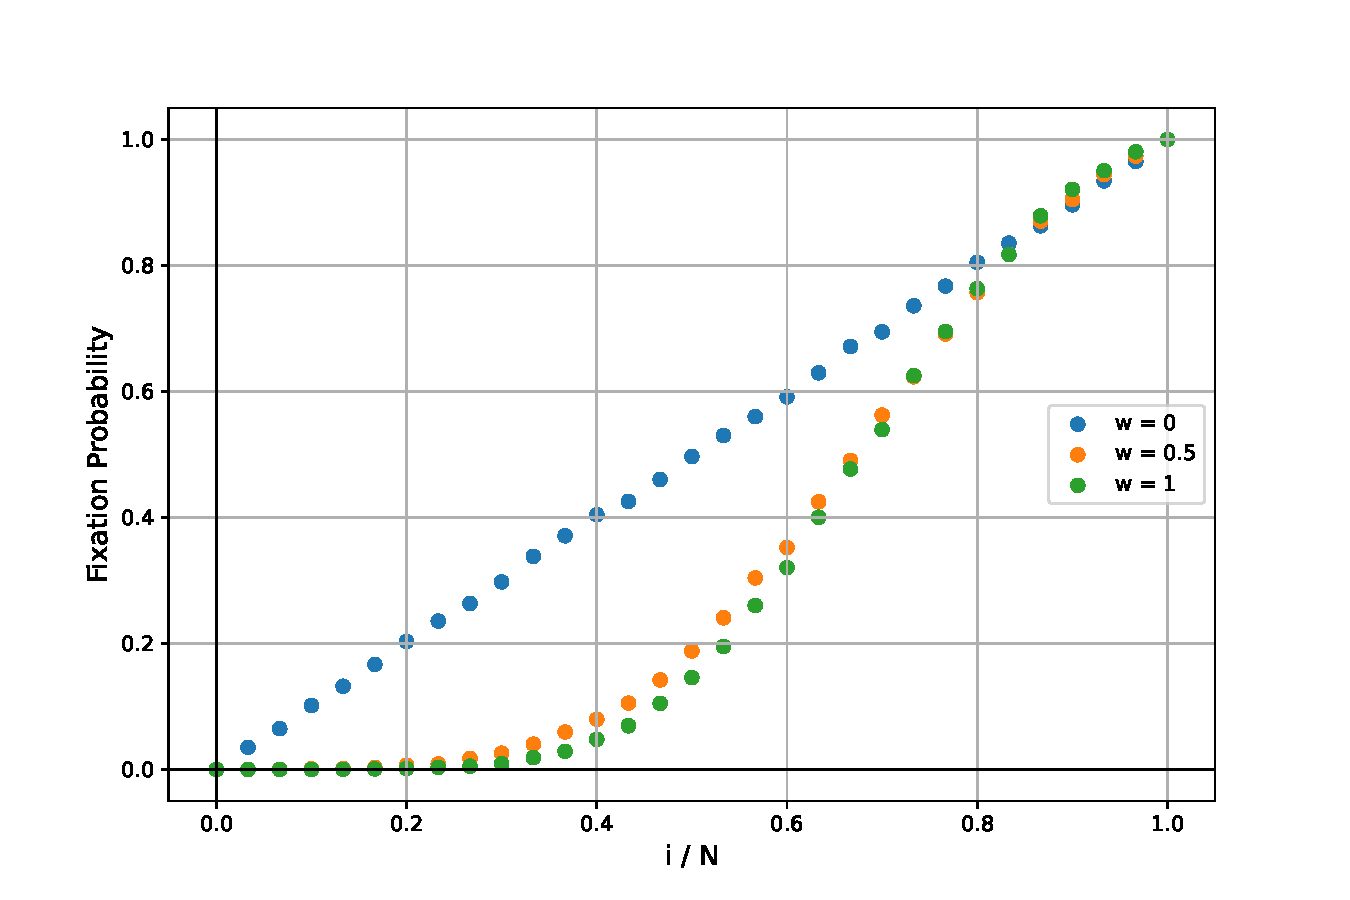
\includegraphics[width=0.8\textwidth]{SH_FP_SIM.pdf}
    \caption{Fixation probability in the Stag Hunt game for a population size $N = 30$, based on $10^4$ simulations. The results correspond to the analytical expression given in equation~\eqref{eq:23}. The $X$-axis represents $i/N$, where $i=$ initial mutant number and $N$ is the population number. The $Y$-axis represents fixation probability.}
    \label{fig:5}
\end{figure}



\subsubsection{Two Players with multiple strategies}
In the previous section we've discussed about the Moran process and fixation probability for  two player two strategy games,
but in this section the aim is to explain the same for the two player multiple strategy games.\\
Let's take the example of Rock-Paper-Scissors game for explaining the Moran process for multiple strategy games.
Suppose,it is a well mixed finite population of fixed size $N$.
Individuals can adopt one of three strategies: Rock(R), Paper(P), Scissors(S).
Number of individuals playing these strategies are $i_R$, $i_P$, $i_S$.
In a $N$ sized finite population, the number of players using each and every strategy should be an integer between $0$ and $N$, and their sum must be exactly $N$. So it can be written that,
\begin{equation}
i_R+i_P+i_S = N \label{eq:36}
\end{equation}
Now, let's write the payoff matrix for the RPS game.
\begin{equation}
\begin{array}{c|ccc}
  & R & S & P \\ \hline
R & 0 & 1 & -1 \\
S & -1 & 0 & 1 \\
P & 1 & -1 & 0
\end{array} \label{eq:37}
\end{equation}
Now let's write the average payoff value for each strategy.
\begin{equation}
\pi_R= i_S - i_P \label{eq:38}
\end{equation}
\begin{equation}
\pi_S= i_P - i_R \label{eq:39}
\end{equation}
\begin{equation}
\pi_P= i_R - i_S \label{eq:40}
\end{equation}
Now the individuals are selected proportional to fitness at birth and proportional to inverse  fitness at death at selection intensity $w$.
Then, the linear fitness for a strategy is $f=1-w+w\pi$.
There are six transition probabilities in each state.
The transition probabilities in each state and to change into one of the six neighbouring states are given by a general equation.
\begin{equation}
T_{Y \to X}(i_R,i_S,i_P)= \frac{i_X f_X}{\sum_Z i_Z f_Z} \cdot \frac{i_Y}{N} \label{eq:41}
\end{equation}
where $X,Y,Z \in (i_R,i_P,i_S)$.\\
Now let's try to write these six transition probabilities,
where each step of the Moran process consists of:
\begin{enumerate}
\item Selection of an individual for reproduction, proportional to fitness.
\item Selection of an individual for death, uniformly at random.
\end{enumerate}
We can write the fitnesses as \( f_R, f_P, f_S \) where,
\begin{align}
f_R &= 1-w+w\pi_R \nonumber\\
f_S &= 1-w+w\pi_S \nonumber\\
f_P &= 1-w+w\pi_P \label{eq:42}
\end{align}
and the total fitness of the population be:
\begin{equation}
\phi = i_R f_R + i_P f_P + i_S f_S \label{eq:43}
\end{equation}
Then, the six transition probabilities are 
\begin{enumerate}
\item Rock reproduces, Paper dies: $T_{P \to R}$.
\begin{align}
T^{R+} &= \frac{i_R f_R}{\phi} \cdot \frac{i_P}{N} \label{eq:44}
\end{align}
\item Paper reproduces, Rock dies: $T_{R \to P}$.
\begin{align}
T^{R-} &= \frac{i_P f_P}{\phi} \cdot \frac{i_R}{N}\label{eq:45}
\end{align}
\item Paper reproduces, Scissors dies: $T_{S \to P}$.
\begin{align}
T^{P+} &= \frac{i_P f_P}{\phi} \cdot \frac{i_S}{N} \label{eq:46}
\end{align}
\item Scissors reproduces, Paper dies: $T_{P \to S}$.
\begin{align}
T^{P-} &= \frac{i_S f_S}{\phi} \cdot \frac{i_P}{N} \label{eq:47}
\end{align}
\item Scissors reproduces, Rock dies: $T_{R \to S}$.
\begin{align}
T^{S+} &= \frac{i_S f_S}{\phi} \cdot \frac{i_R}{N} \label{eq:48}
\end{align}
\item Rock reproduces, Scissors dies: $T_{S \to R}$.
\begin{align}
T^{S-} &= \frac{i_R f_R}{\phi} \cdot \frac{i_S}{N} \label{eq:49}
\end{align}
\item Everyone stays at the same state:
\begin{align}
T_{\text{Stay}}(i_R,i_P,i_S) = T_{R \to R} + T_{S \to S} + T_{P \to P} \label{eq:50}
\end{align}
\end{enumerate}
All six of these transition probabilities completely determine the stochastic dynamics of the Moran process of a three-strategy game such as Rock-Paper-Scissors.
The population will move to any one of the six neighbouring states at each time step in the strategy simplex, which means it will move to a state where one strategy will be increased and another decreased by $1$ person.
The development of this system is a Markov chain process over the state space of all feasible $(i_R, i_P, i_S)$ triplets fulfilling equation \eqref{eq:36}.
This process continues until it arrives at one of the absorbing boundaries, which means only one strategy remains and all other strategies become extinct.
These absorbing states can be equated to fixation of single strategy.
\begin{figure}[H]
    \centering
    \includegraphics[width=0.8\textwidth]{Fixation_RPS.pdf}
    \caption{In a finite population of size of $N = 33$ with $ 10^4$ simulations and a zero-sum RPS payoff matrix \eqref{eq:36}, the fixation probability of Rock is highest near the Rock-rich corner. Under strong selection $w=1$, fixation is determined primarily by payoff advantages rather than initial frequency alone. Near the Rock-rich corner, Rock not only has a numerical advantage but also gains high fitness from frequent wins against Scissors, enabling it to dominate and fixate with high probability and the same explanation goes for the other two strategies present.}
    \label{fig:6}
\end{figure}

\subsection{Evolutionary Dynamics of Structured Populations}
In the previous subsection, we tried to explain the evolutionary dynamics using stochastic process in a finite population, but the population was unstructured. But to make the mathematical process and our understanding about the evolutionary dynamics more realistic, we have to consider a structured finite population.
The structure of a population can influence the evolutionary dynamics in biological systems. For an example, in a paper by Arne Traulsen, it was discussed that the structure of a microbial population can influence it's evolutionary dynamics \citep{Traulsen2021}.\\
Now, how to do that mathematically? One of the most popular and common theory to model and understand the structure of a population is evolutionary graph theory \citep{Lieberman2005}. 
In the graph theory the nodes represent individuals and the links determines the individual's neighbours, and where an individual can place it's offspring. But to know which individual will reproduce and how the offspring will be placed, we need to understand update mechanism.
The two most important events that determine and control the population dynamics are birth and death. Based on these two events, the selection type is often determined whether it's local selection or global selection and ultimately it influence the structure of the population.
For birth we use $b$ if the birth is random and $B$ if the birth is chosen with the probability proportional to it's selection parameter.
For death we use $d$ if the death is random and $D$ if the death is chosen with the probability proportional to it's selection parameter.
According to this, we can write eight update mechanisms $bd$, $db$, $Bd$, $dB$, $Db$, $bD$, $BD$, $DB$.\\
Now let's try to understand the $Bd$ rule, suppose we are applying $Bd$ rule in a population size of $N$, where there are $n$ mutants and $N-n$ wild types, with mutants having a relative selection parameter for birth $r$ with respect to the wild types.\\
Suppose, the mutant number of the population is increased by $1$, means one mutant is selected for reproduction, it's a global selection as the mutant is selected from the whole population.
Now, one from the neighbours of the reproductive mutant is selected for death, it is a local selection event.\\
Now, the transition probability of mutant number being increased by one is:
\begin{equation}
T_{Bd}^+ = \frac{rn}{rn+ N-n} \cdot \frac{N-n}{N-1} \label{eq:51}
\end{equation}
In a similar manner, the transition probability of mutant number being decreased by one is:
\begin{equation}
T_{Bd}^- = \frac{N-n}{rn+ N-n} \cdot \frac{n}{N-1} \label{eq:52}
\end{equation}
From these two equations we can write $T_{Bd}^-/T_{Bd}^+ = 1/r$. So the fixation probability will be:
\begin{equation}
\frac{1+\sum_{i=1}^{n-1}\prod_{j=1}^i \frac{T_{Bd}^-}{T_{Bd}^+}}{1+ \sum_{i=1}^{N-1}\prod_{j=1}^i \frac{T_{Bd}^-}{T_{Bd}^+}} = \frac{\frac{1-\frac{1}{r^n}}{1-r}} {\frac{1-\frac{1}{r^N}}{1-r}} = \frac{1-\frac{1}{r^n}}{1-\frac{1}{r^N}} \label{eq:53}
\end{equation}
If we try to write the dB update mechanism, the transition probabilities will be:
\begin{align}
T_{dB}^+ &= \frac{N-n}{N} \cdot \frac{rn}{rn+N-r-1} \nonumber\\
T_{dB}^- &= \frac{n}{N} \cdot \frac{N-n}{(n-1)r + N-n} \label{eq:54}
\end{align}
Then, the fixation probability is:
\begin{equation}
\rho_n = \frac{1 + \sum_{i=1}^{n-1} \prod_{j=1}^i[ r^{-1} \cdot \frac{(n-1)r + N - n}{n r + N - n - 1}]}{1 + \sum_{i=1}^{N-1} \prod_{j=1}^i[ r^{-1} \cdot \frac{(n-1)r + N - n}{n r + N - n - 1}]} \label{eq:55}
\end{equation}
\subsubsection{Two-player game with two strategies in Structured Population}
As discussed earlier in the subsubsection \ref{subsubsec:Two-player games with two strategies} of the subsection \ref{subsec:Replicator Dynamics}, stag hunt game is a classical example of game theory to understand the interplay between risk and trust. There are two strategies, cooperation and defection. The stag hunt game can be used to model how cooperation can persist when cooperators cluster locally in structured finite populations like biofilms, among microbial population \citep{Lambert2014}. 
The simplest way to simulate a game in structured population through graphs is simulating the game in square lattice spatial structure.\\
Let's write the payoff matrix for the stag hunt game,
\begin{equation}
\begin{array}{c|cc}
   & \text{Cooperate (C)} & \text{Defect (D)} \\
  \hline
  \text{Cooperate (C)} & S = 4 & S = 1 \\
  \text{Defect (D)} & H = 3 & H = 3 \\
\end{array} \label{eq:56}
\end{equation}
Now, on a square lattice the payoff of the strategy of an individual depends on the neighbours of the individual, where the number of cooperative neighbours is denoted as $n_C$ and number of the defective neighbours is denoted by $n_D$. \\
Average payoff of the individual playing cooperation strategy is:
\begin{equation}
\pi_C = n_C \cdot 4 + n_D \cdot 1 \label{eq:57}
\end{equation}
and the average payoff of the individual playing defection is:
\begin{equation}
\pi_D = n_C \cdot 3 + n_D \cdot 3 \label{eq:58}
\end{equation}
Then, the fitness is respectively, $f_C = 1 - w + w \cdot \pi_C$ and $f_D = 1 - w + w \cdot \pi_D$.
then, the relative fitness of mutants for birth with respect to the wild types can be analytically represented as:
\begin{equation}
r = \frac{f_C}{f_D} = \frac{1 - w + w \cdot \pi_C}{1 - w + w \cdot \pi_D} \label{eq:59}
\end{equation}
Now, if we apply the $Bd$ update mechanism in a population size of $N$, where there are $n$ mutants (cooperators) and $N_n$ wild types (defectors). Then, the transition probability of mutant number being increased by one and the transition probability of mutant number being decreased by one can be calculated using the equation \eqref{eq:50} and \eqref{eq:51}, where r = relative fitness = $\frac{1 - w + w \cdot \pi_C}{1 - w + w \cdot \pi_D}$. Now, we can calculate the fixation probability using the equation \eqref{eq:52}.
\begin{figure}[H]
    \centering
    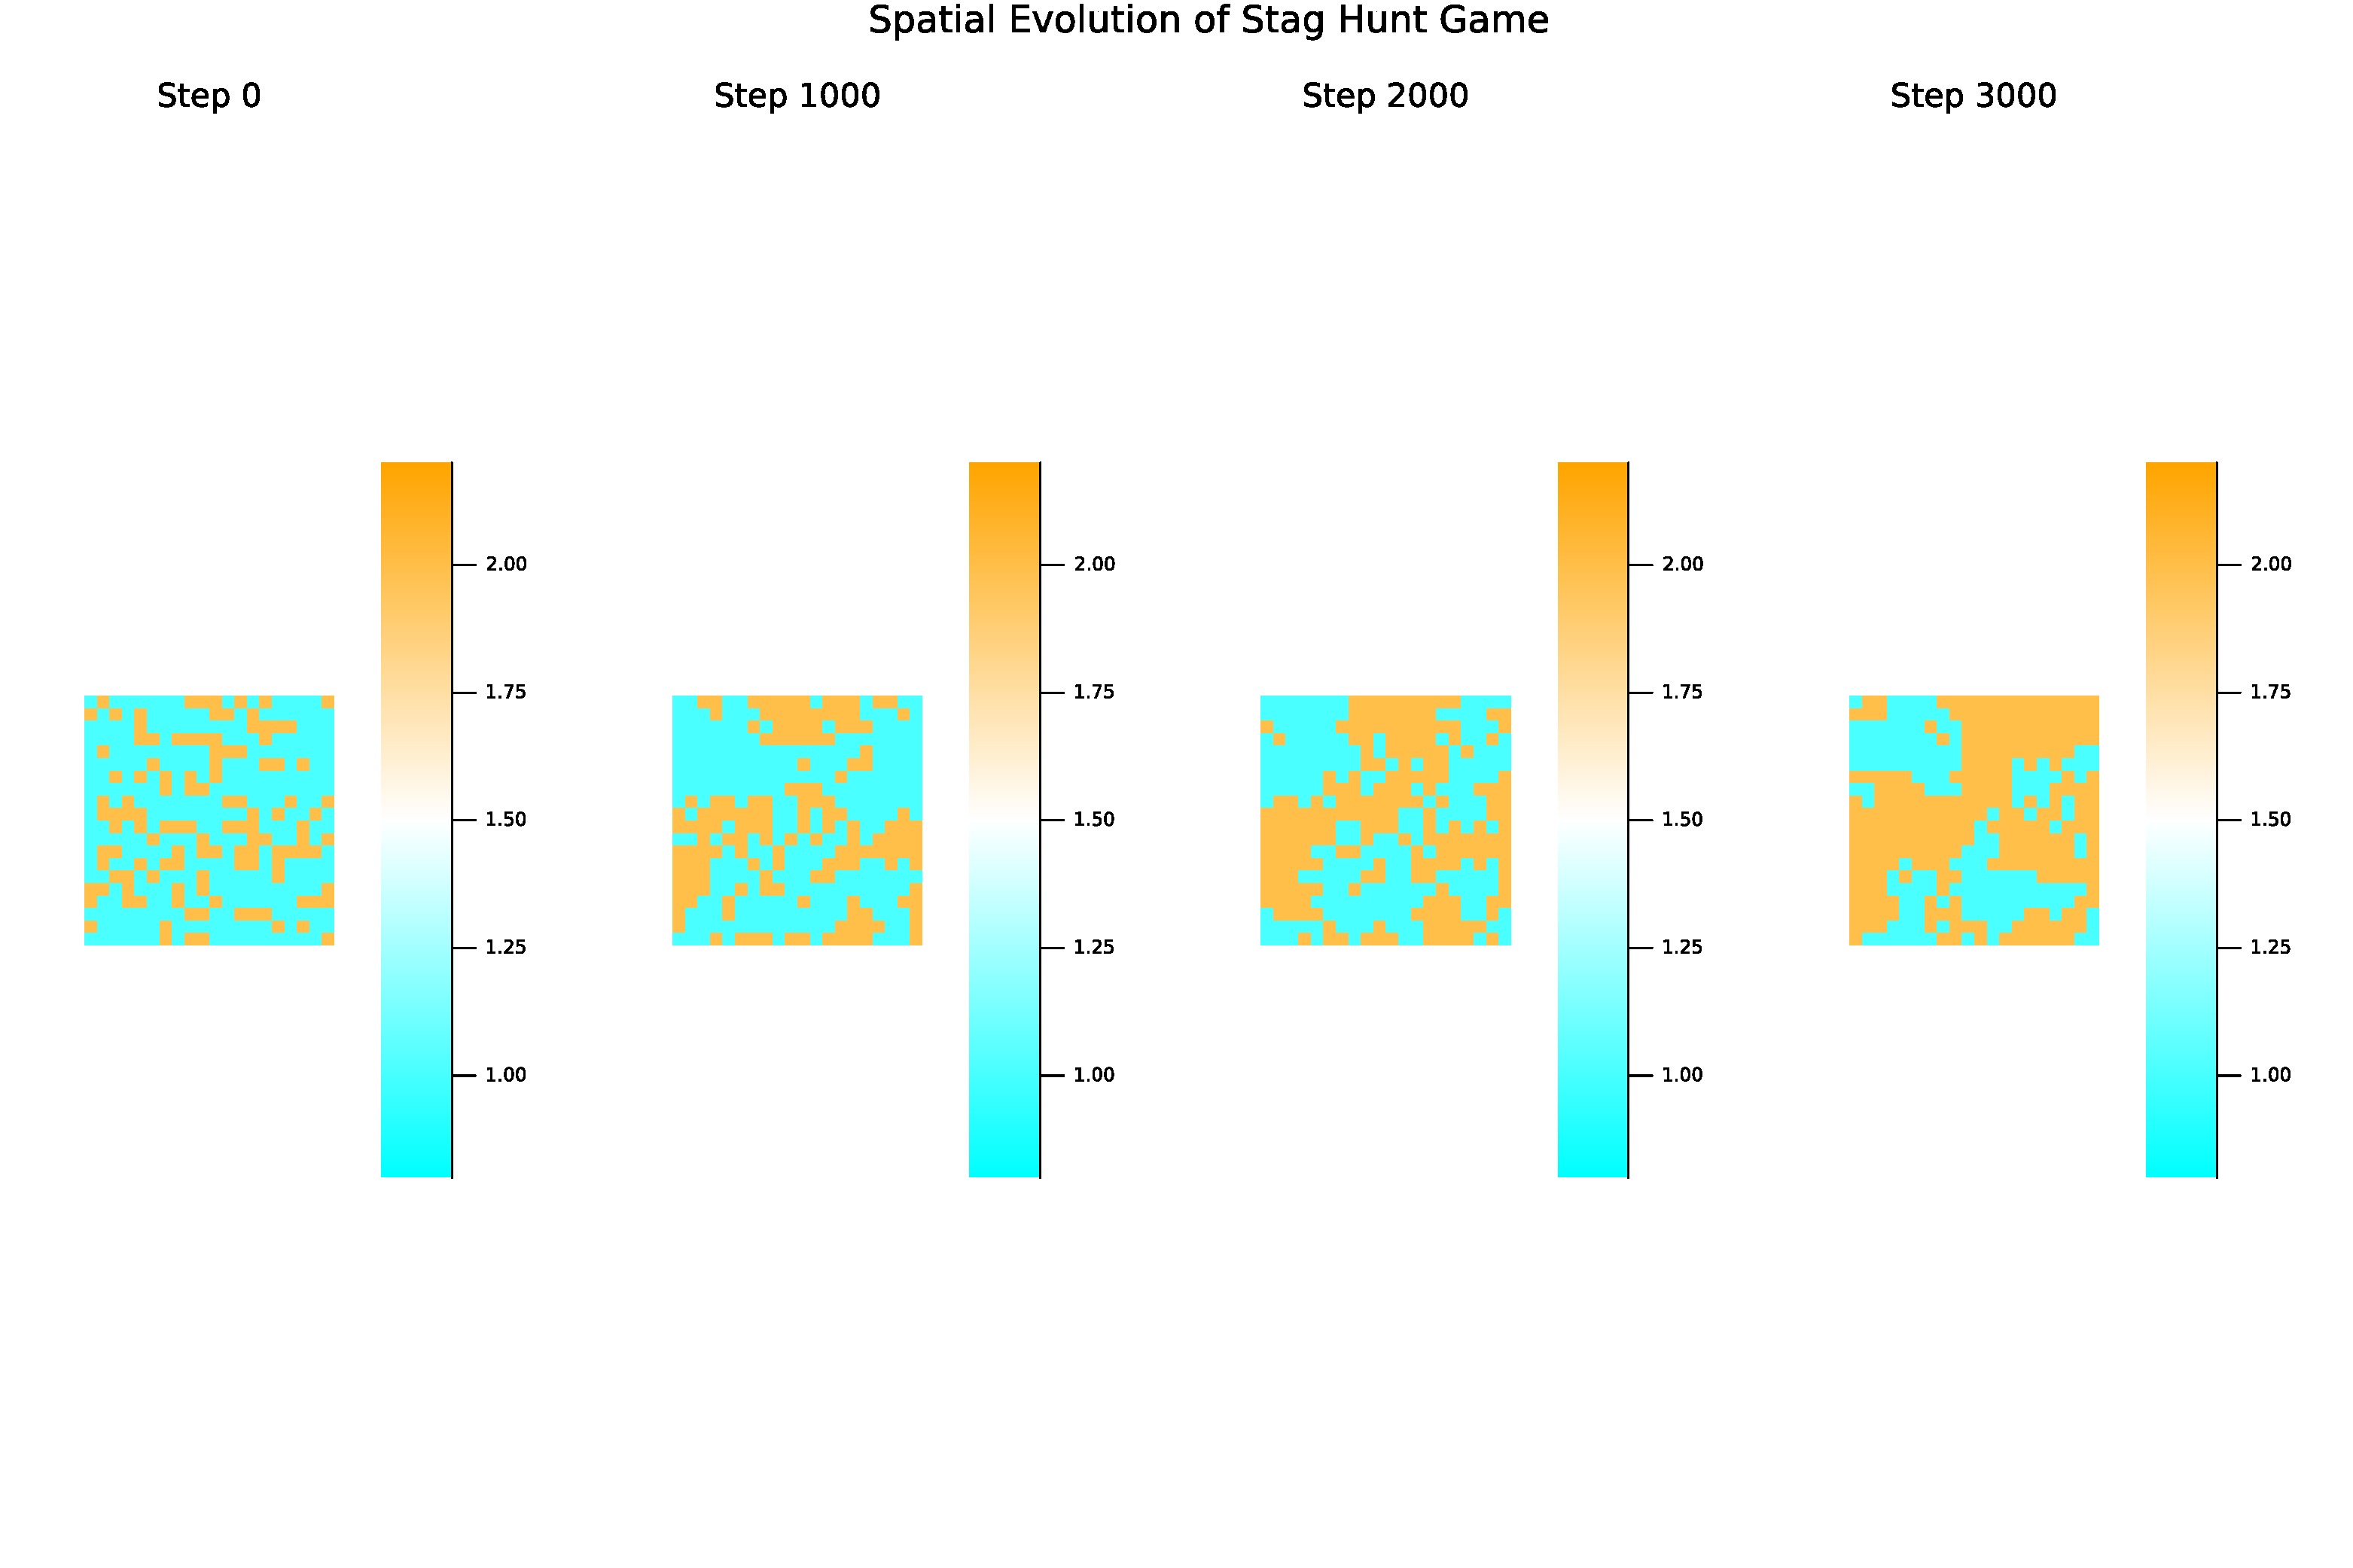
\includegraphics[width=0.8\textwidth]{SH_SP.pdf}
    \caption{Spatial evolution of the stag hunt game, over four time steps. Where the orange color denotes the defectors and the cyan color the cooperators.
    At time step $0$, the cooperators are $300\%$ and defectors are $70\%$. 
    At time step $1000$, the cooperators are $34.3\%$ and defectors are $65.7\%$. 
    At time step $2000$, cooperators are $37.1\%$ and defectors are $62.9\%$. 
    At time step $3000$, the cooperators are $42.9\%$ and defectors are $57.1\%$.}
    \label{fig:6}
\end{figure}
Now, we have simulated the stag-hunt game on square-lattice with Moore neighbourhood. Square lattice is the easiest way to construct a structured population. Apart from it, many networks are said to have small-world properties, in other words, the network of any two of their members can be communicated with each other via a small number of linkages (steps). Thus, the Newman-Watts-Strogatz (NWS) algorithm generates a small-world network, which is executed in this study. This algorithm initially forms a d-dimensional lattice,in our case $d=1$.  Then, each vertex is drawn an edge with probability $\beta$.  The average path length between any two vertices in a NWS network is very small and the clustering coefficient is very high.
In this study we tried to simulate the stag hunt game with same conditions like in sqaure lattice on NWS network.
\begin{figure}[ht]
  \centering
  \begin{subfigure}[b]{0.45\textwidth}
    \centering
    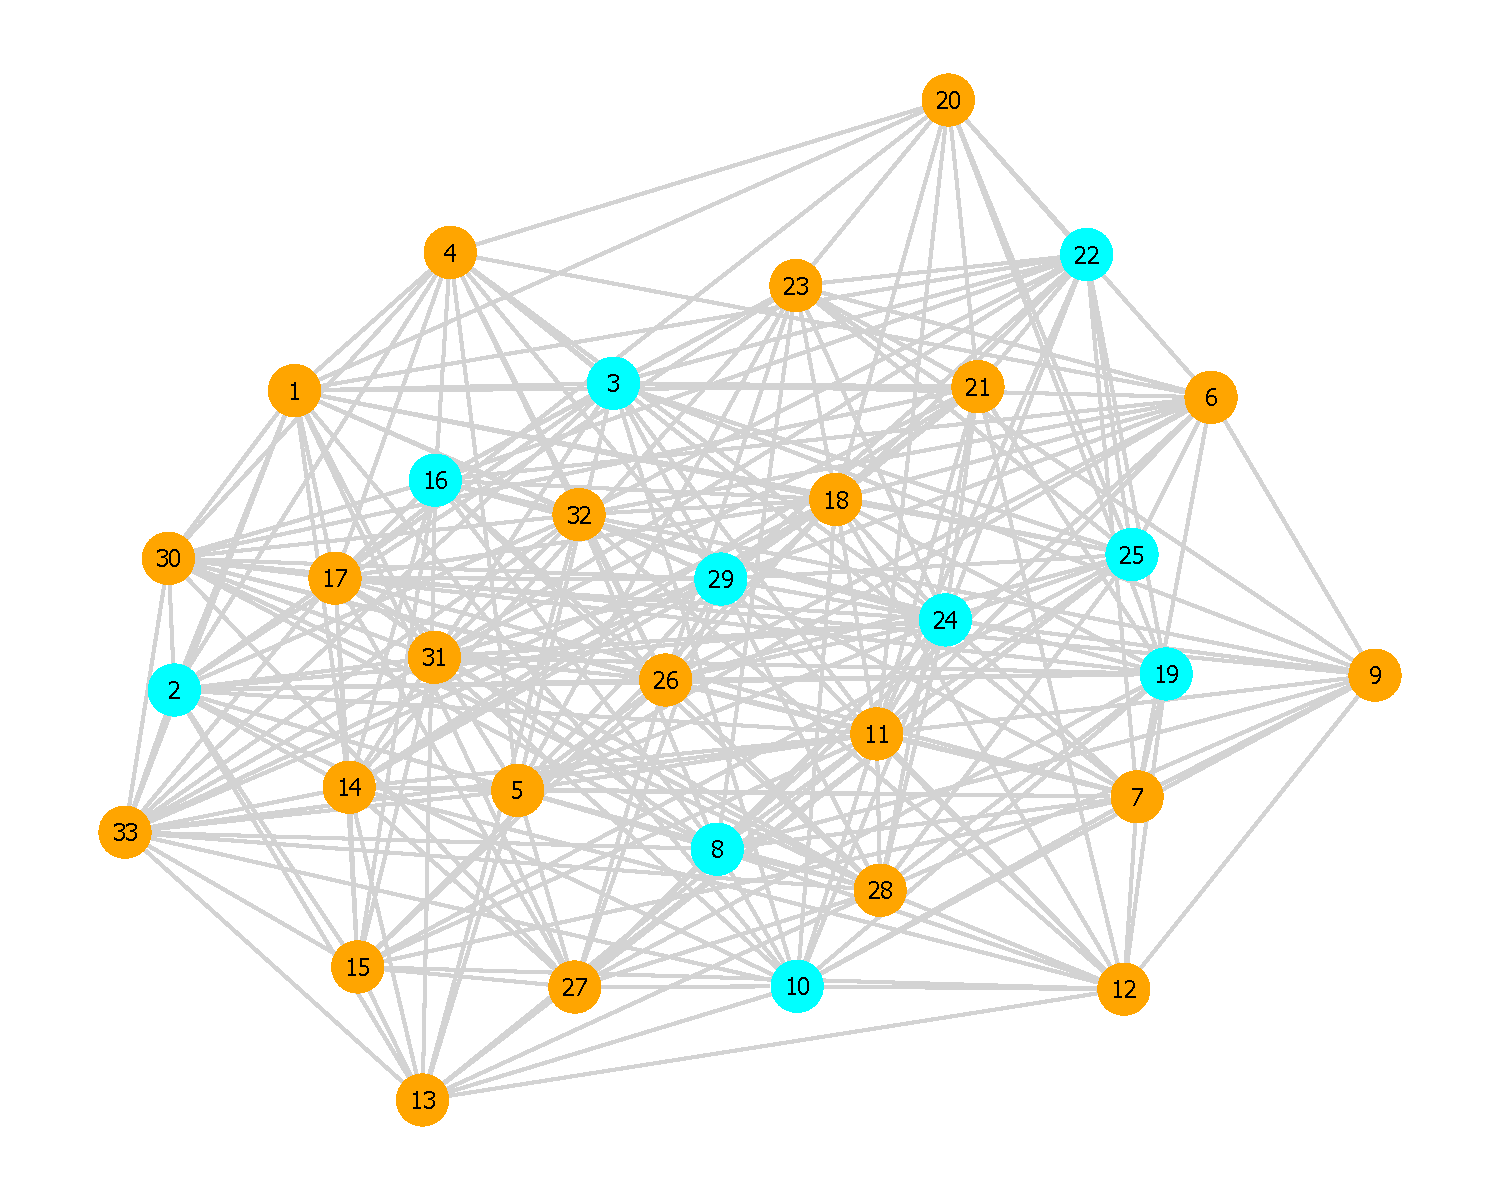
\includegraphics[width=\textwidth]{SH_WS_step_0.pdf}
    \caption{This is the NWS network at step $0$, with initial condition, where there is $30\%$ cooperator and $70\%$ defector.}
    \label{fig:fig8}
  \end{subfigure}
  \hfill
  \begin{subfigure}[b]{0.45\textwidth}
    \centering
    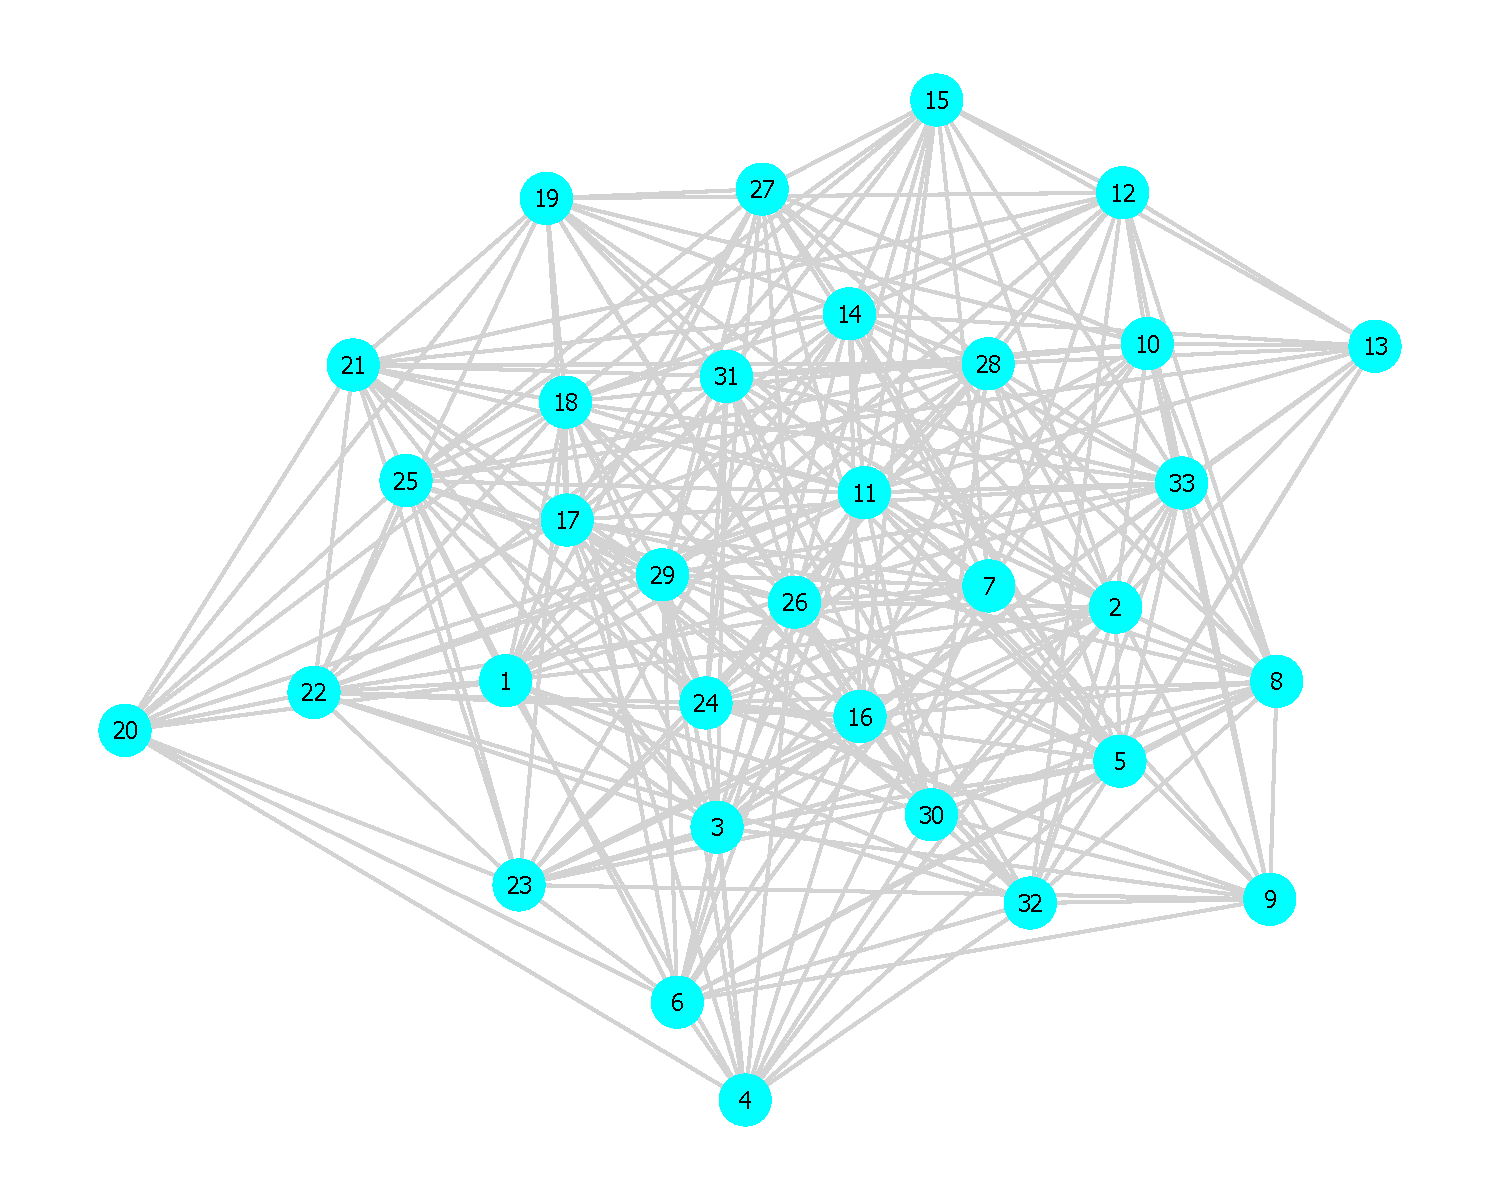
\includegraphics[width=\textwidth]{SH_WS_final_step.pdf}
    \caption{This is the NWS network at step $381$,where the cooperators fixed the population.}
    \label{fig:fig2}
  \end{subfigure}
  \caption{This figure shows the simulation of Stag Hunt game in Newman-Watts-Strogatz network, with payoff strcuture \eqref{eq:6}, and the network construction conditions are N(nodes)= $33$, k = neighbours per node in ring lattice = $6$, and probability $\beta = 0.4$. The initial conditions for the network is randomly placed $30\%$ cooperator in a defector world. So, at the initial step, there was $10$ cooperators and $23$ defectors, in the $381$ step, the cooperators fixed the population.Here, orange= defector and cyan= cooperator.}
  \label{fig:side_by_side}
\end{figure}







\section{Results}
\section{Discussion}





\textbf{Code availability}.
Appropriate computer code describing the model is available at 
\texttt{ REDACTED for review}.% {\url{https://github.com/tecoevo/beliefs}}.

\section{Acknowledgements}
\texttt{ REDACTED for review}.% {\url{https://github.com/tecoevo/beliefs}}.


\bibliographystyle{naturemag}
\bibliography{references.bib}

\renewcommand{\theequation}{SI.\arabic{equation}}
\setcounter{equation}{0}

\renewcommand{\thefigure}{SI.\arabic{figure}}
\setcounter{figure}{0}

\section{Supplementary material}


\subsection{Analysis of the simple system}




\end{document}
